\section{Auswertung}
\label{sec:Auswertung}
\subsection{statistische Methode}

Der Abstand der Thermoelemente zueinander beträgt jeweils $\Delta x=3\,\si{\centi\meter}$.


\begin{figure}[H]
  \centering
  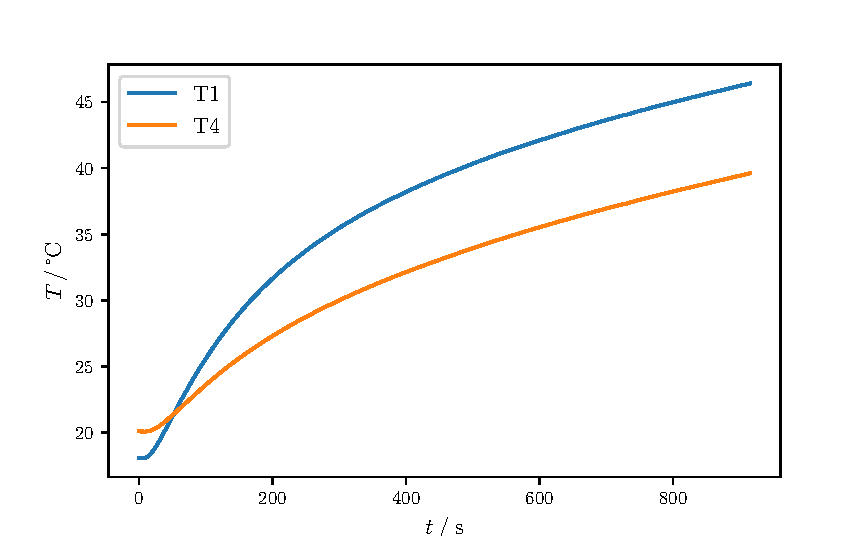
\includegraphics{plot1.pdf}
  \caption{Zeitlicher Temperaturverlauf des breiten und dünnen Messingstabes bei der statischen Methode}
  \label{fig:a}
\end{figure}

\begin{figure}[H]
  \centering
  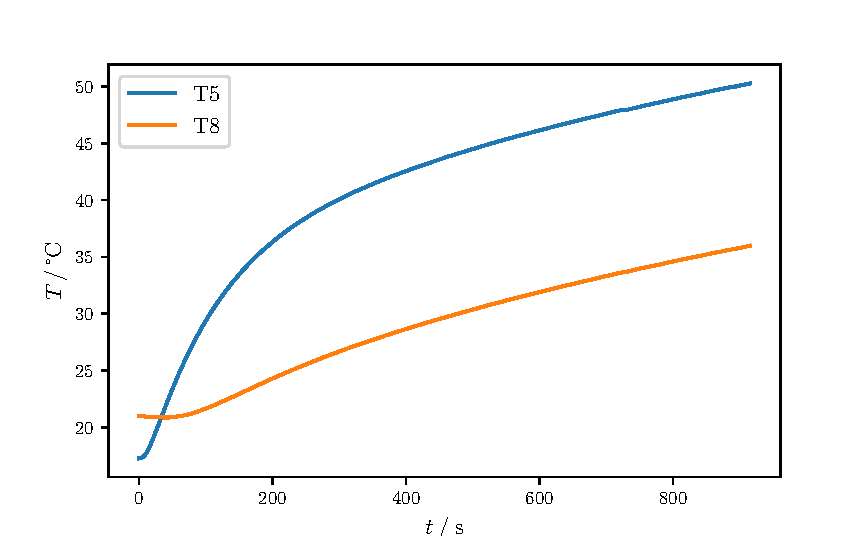
\includegraphics{plot2.pdf}
  \caption{Zeitlicher Temperaturverlauf des Aluminium- und Edelstahlstabes bei der statischen Methode}
  \label{fig:b}
\end{figure}

\noindent In Abbildung \ref{fig:a} sind die Temperaturverläufe der beiden Messingstäbe aufgetragen. Dabei fällt auf, dass der breite Stab schneller
wärmer wird als der dünne Stab und sich auf lange Sicht eine Temperaturdifferenz von ca $7\,\si{\celsius}$ einstellt. Auch wenn 
der dünne Messingstab zu Beginn der Messung eine höhere Starttemperatur von $20,1\,\si{\celsius}$ als der breite Messingstab ($18,07\,\si{\celsius}$) hatte, so wurde
diese Temperaturdifferenz bereits nach 45 Sekunden ausgeglichen.


\noindent In Abbildung \ref{fig:b} sind die Temperaturverläufe des Aluminiumstabes und des Edelstahlstabes aufgetragen. Hierbei
wird der Aluminiumstab schneller heiß als der Edelstahlstab. Die Temperaturdifferenz stellt sich auf lange Sicht bei ca $14\,\si{\celsius}$ ein. Auch wenn 
der Edelstahlstab zu Beginn der Messung eine höhere Starttemperatur von $21,01\,\si{\celsius}$ als der Aluminiumstab ($17,27\,\si{\celsius}$) hatte, so wurde
diese Temperaturdifferenz sogar schon nach nach 35 Sekunden ausgeglichen.


\noindent Generell lässt sich sagen, dass alle Temperaturverläufe ihren größten Anstieg in den ersten 200 Sekunden haben. Dabei steigt die
Temperatur des Aluminiums schon nach den ersten Sekunden stark an, während Edelstahl sich erst nach einer Minute merkbar erwärmt.
Um beurteilen zu können, welcher Stab die beste Wärmeleitung hat, werden die Temperaturen nach 700 Sekunden verglichen (Siehe Tabelle \ref{tab:a}).

\begin{table}[H]
\centering
\caption{Temperatur der Thermoelemente nach 700 Sekunden}
\label{tab:a}
\sisetup{table-format=1.2}
\begin{tabular}{S[table-format=3.0] S S[table-format=3.2]}
\toprule
{Thermoelement} & {$T\,/\,\si{\celsius}$}\\
\midrule
T1 & 43,62\\
T4 & 36,94\\
T5 & 47,62\\
T8 & 33,32\\

\bottomrule
\end{tabular}
\end{table}

\noindent Es lässt sich also sagen, dass der Aluminiumstab die beste Wärmeleitung hat.\\


\noindent In den Abbildungen \ref{fig:c} und \ref{fig:d} sind die Temperaturdifferenzen des nahen und fernen Thermoelementes des breiten
Messingstabes und des Edelstahlstabes gegen die Zeit aufgetragen.
\begin{figure}[H]
  \centering
  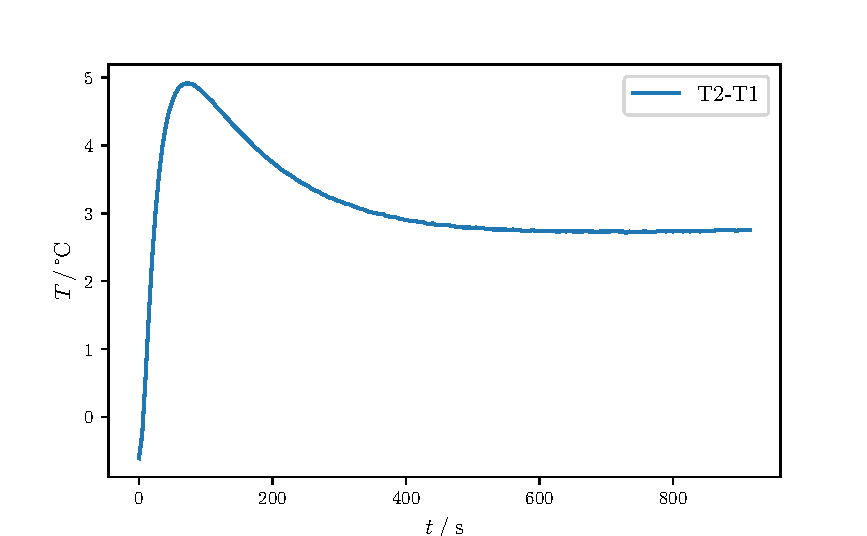
\includegraphics{diff1.pdf}
  \caption{Zeitlicher Verlauf der Temperaturdifferenz zwischen T1 und T2 am Messingstab bei der statischen Methode}
  \label{fig:c}
\end{figure}

\begin{figure}[H]
  \centering
  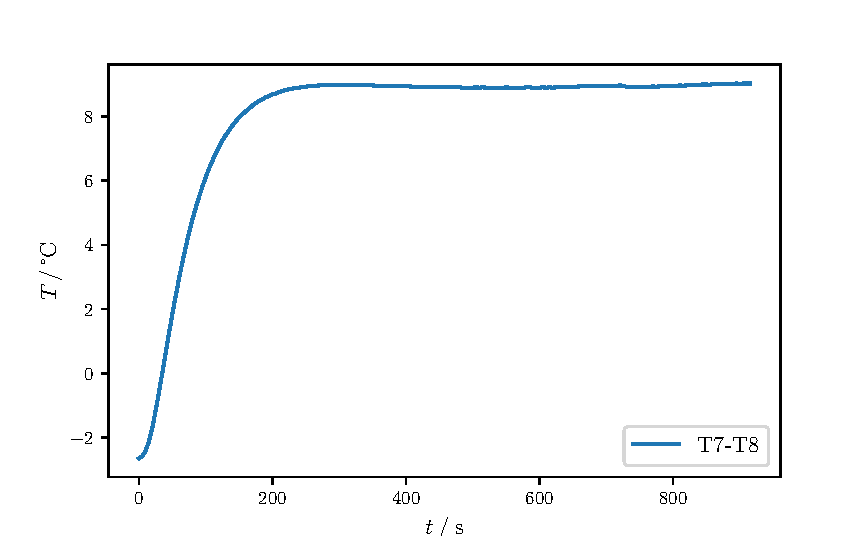
\includegraphics{diff2.pdf}
  \caption{Zeitlicher Verlauf der Temperaturdifferenz zwischen T7 und T8 am Edelstahstab bei der statischen Methode}
  \label{fig:d}
\end{figure}

\noindent Beide Verläufe nähern sich nach einiger Zeit einem festen Wert an. Die Temperaturdifferenz beim Messingstab
stellt sich nach ca 400 Sekunden auf  $2,8\,\si{\celsius}$ ein und die des Edelstabstabes nach schon 200 Sekunden auf $9,5\si{\celsius}$.
Der größte Unterschied zwischen den beiden Graphen ist der, dass die Temperaturdifferenz des Messingstabes zunächst auf $5\,\si{\celsius}$ ansteigt, bevor sich der
gleichbleibende Wert einspielt. Beim Messingstab nähert sich der Graph von unten seiner oberen Schranke an und überschreitet diese nicht.


\subsection{Dynamische Methode}
In den Abbildungen \ref{fig:e}, \ref{fig:f} und \ref{fig:g} sind die zeitlichen Temperaturverläufe des breiten Messingstabes, des Aluminiumstabes und des Edelstahlstabes vom nahen und fernen Thermoelement aufgetragen.
Um daraus die Amplituden A1 und A2, sowie die Phasendifferenzen $\Delta t$ zu bestimmen, werden alle Hoch- und Tiefpunkte aus den Messdaten abgelesen (siehe Tabelle \ref{tab:b}, \ref{tab:c} und \ref{tab:d}).
Die tatsächlichen Amplituden werden dann nach der Formel

\begin{equation}
  A_n=\frac{Max_n-\frac{Min_n+Min_{n+1}}{2}}{2}
  \label{eq:a}
\end{equation}

\noindent berechnet. Zum letzten Maximum kann jedoch keine Amplitude bestimmt werden, da diese kein dazugehöriges zweites Minimum hat.
Die Phasendifferenz kann dann mit den Formeln für den Mittelwert

\begin{equation}
  \bar{x}=\frac{1}{n} \cdot \sum_{i=1}^n x_i
  \label{eq:b}
\end{equation}

\noindent und den Standardfehler des Mittelwertes

\begin{equation}
  \Delta\bar{x}=\sqrt{\frac{1}{n(n-1)}\cdot \sum_{i=1}^n(x_i-\bar{x})^2}
  \label{eq:c}
\end{equation}

\noindent aus den einzelnen Zeitabständen $\delta t$ zwischen den Maxima der Graphen bestimmt werden.

\subsubsection{Breiter Messingstab}

\begin{figure}[H]
  \centering
  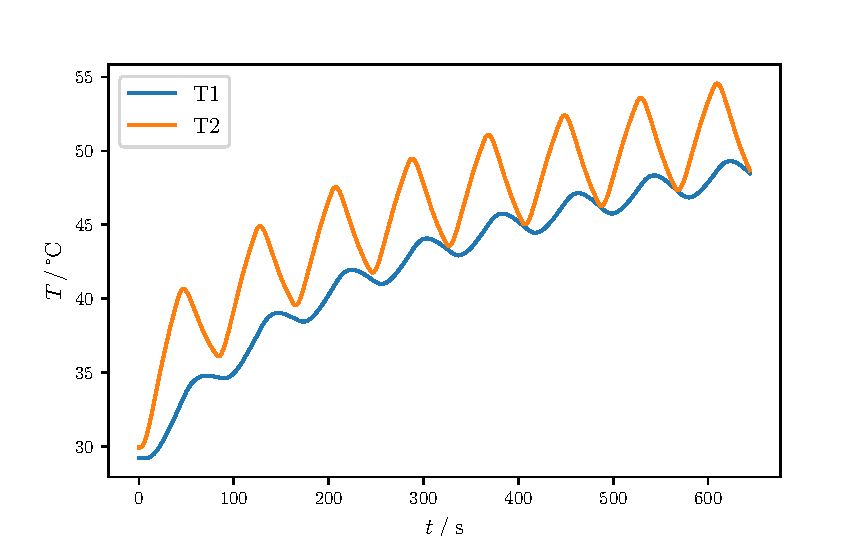
\includegraphics{plot3.pdf}
  \caption{Zeitlicher Temperaturverlauf von T1 und T2 am Messingstab bei der dynamischen Methode}
  \label{fig:e}
\end{figure}

  \begin{table}[H]
  \centering
    \begin{subtable}{.42\linewidth}
      \centering
        \csvreader[tabular=c c|c c|,
    head=false, 
    table head= $t\:/\:\si{\second}$ & $T_{Max}\:/\:\si{\celsius}$ & $t\:/\:\si{\second}$ & $T_{Min}\:/\si{\celsius}$\\\midrule,
    late after line= \\]
    {content/Data/Tab1.csv}{1=\eins, 2=\zwei, 3=\drei, 4=\vier}{$\num{\eins}$ & $\num{\zwei}$ & $\num{\drei}$ & $\num{\vier}$}
            \caption{Extrema bei T1}

    \end{subtable}
    \begin{subtable}{.42\linewidth}
      \centering
        \csvreader[tabular=|c c|c c,
    head=false, 
    table head= $t\:/\:\si{\second}$ & $T_{Max}\:/\:\si{\celsius}$ & $t\:/\:\si{\second}$ & $T_{Min}\:/\si{\celsius}$\\\midrule,
    late after line= \\]
    {content/Data/Tab2.csv}{1=\eins, 2=\zwei, 3=\drei, 4=\vier}{$\num{\eins}$ & $\num{\zwei}$ & $\num{\drei}$ & $\num{\vier}$}
           \caption{Extrema bei T2}

    \end{subtable} 
        \caption{Extrema der Temperaturen beim breiten Messingstab bei der dynamischen Methode}
    \label{tab:b}
\end{table}


\noindent Die Amplituden ergeben sich durch Gleichung \ref{eq:a} zu den Werten in Tabelle \ref{tab:aa}.
 
 
 \begin{table}[H]
  \centering
    \begin{subtable}{.42\linewidth}
      \centering
        \csvreader[tabular=c c,
    head=false, 
    table head= Amplitude & $T_{Max}\:/\:\si{\celsius}$\\\midrule,
    late after line= \\]
    {content/Data/Tab1_1.csv}{1=\eins, 2=\zwei}{$\num{\eins}$ & $\num{\zwei}$}
            \caption{Amplituden von T1}

    \end{subtable}
    \begin{subtable}{.42\linewidth}
      \centering
        \csvreader[tabular=c c,
    head=false, 
    table head= Amplitude & $T_{Max}\:/\:\si{\celsius}$ \\\midrule,
    late after line= \\]
    {content/Data/Tab1_2.csv}{1=\eins, 2=\zwei}{$\num{\eins}$ & $\num{\zwei}$}
           \caption{Amplituden von T2}

    \end{subtable} 
        \caption{Amplituden der Temperatur des breiten Messingstabes}
    \label{tab:aa}
\end{table}
\noindent Diese lassen sich nun mit \ref{eq:b} und \ref{eq:c} als 

\begin{equation*}
  A_{fern}=(1,13 \pm 0,07)\,\si{\celsius} 
\end{equation*}
\noindent und
\begin{equation*}
  A_{nah}=(3,49 \pm 0,07)\,\si{\celsius} 
\end{equation*}
\noindent schreiben. Die einzelnen $\delta t$ werden in Tabelle \ref{tab:aaa} aufgeführt.


\begin{table}[H]
      \centering
        \csvreader[tabular=c c,
    head=false, 
    table head= Phasendifferenz & $t\:/\:\si{\second}$\\\midrule,
    late after line= \\]
    {content/Data/Tab1_3.csv}{1=\eins, 2=\zwei}{$\num{\eins}$ & $\num{\zwei}$}

        \caption{Phasendifferenz der Temperaturmaxima beim breiten Messingstab}
    \label{tab:aaa}
\end{table}


\noindent Für $\Delta t$ gilt dann mit \ref{eq:b} und \ref{eq:c}

\begin{equation*}
  \Delta t=(16,1\pm1,3)\,\si{\second}
\end{equation*}

\noindent Um nun die Wärmeleitfähigkeit mit Gleichung \ref{eq:kappa} zu bestimmen wurde $\rho=8,4\,\si{\gram\per\centi\meter\tothe{3}}$ und $c=377\,\si{\joule\per\kilo\gram\per\kelvin}$ (siehe \cite{chemieMessing}) angenommen.
Daraus ergibt sich dann insgesamt

\begin{equation*}
  \kappa=(78\pm8)\,\si{\watt\per\meter\per\kelvin}.
\end{equation*}

\subsubsection{Aluminiumstab}

\begin{figure}[H]
  \centering
  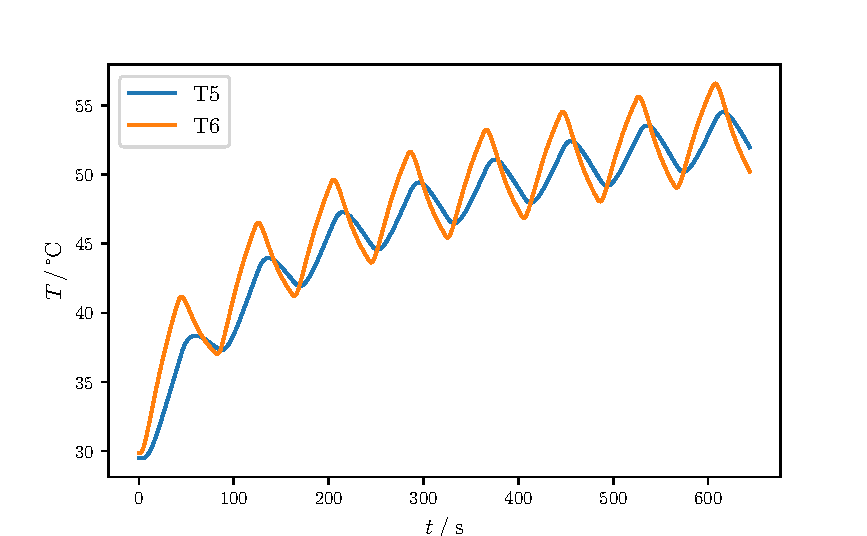
\includegraphics{plot4.pdf}
  \caption{Zeitlicher Temperaturverlauf von T1 und T2 am Messingstab bei der dynamischen Methode}
  \label{fig:f}
\end{figure}


  \begin{table}[H]
  \centering
    \begin{subtable}{.42\linewidth}
      \centering
        \csvreader[tabular=c c|c c|,
    head=false, 
    table head= $t\:/\:\si{\second}$ & $T_{Max}\:/\:\si{\celsius}$ & $t\:/\:\si{\second}$ & $T_{Min}\:/\si{\celsius}$\\\midrule,
    late after line= \\]
    {content/Data/Tab3.csv}{1=\eins, 2=\zwei, 3=\drei, 4=\vier}{$\num{\eins}$ & $\num{\zwei}$ & $\num{\drei}$ & $\num{\vier}$}
            \caption{Extrema bei T5}

    \end{subtable}
    \begin{subtable}{.42\linewidth}
      \centering
        \csvreader[tabular=|c c|c c,
    head=false, 
    table head= $t\:/\:\si{\second}$ & $T_{Max}\:/\:\si{\celsius}$ & $t\:/\:\si{\second}$ & $T_{Min}\:/\si{\celsius}$\\\midrule,
    late after line= \\]
    {content/Data/Tab4.csv}{1=\eins, 2=\zwei, 3=\drei, 4=\vier}{$\num{\eins}$ & $\num{\zwei}$ & $\num{\drei}$ & $\num{\vier}$}
           \caption{Extrema bei T6}

    \end{subtable} 
        \caption{Extrema der Temperaturen beim Aluminiumstab bei der dynamischen Methode}
    \label{tab:c}
\end{table}

\noindent Die Amplituden ergeben sich durch Gleichung \ref{eq:a} zu den Werten in Tabelle \ref{tab:bb}.
 
 
 \begin{table}[H]
  \centering
    \begin{subtable}{.42\linewidth}
      \centering
        \csvreader[tabular=c c,
    head=false, 
    table head= Amplitude & $T_{Max}\:/\:\si{\celsius}$\\\midrule,
    late after line= \\]
    {content/Data/Tab2_1.csv}{1=\eins, 2=\zwei}{$\num{\eins}$ & $\num{\zwei}$}
            \caption{Amplituden von T5}

    \end{subtable}
    \begin{subtable}{.42\linewidth}
      \centering
        \csvreader[tabular=c c,
    head=false, 
    table head= Amplitude & $T_{Max}\:/\:\si{\celsius}$ \\\midrule,
    late after line= \\]
    {content/Data/Tab2_2.csv}{1=\eins, 2=\zwei}{$\num{\eins}$ & $\num{\zwei}$}
           \caption{Amplituden von T6}

    \end{subtable} 
        \caption{Amplituden der Temperatur des Aluminiumstabes}
    \label{tab:bb}
\end{table}

\noindent Diese lassen sich nun mit \ref{eq:b} und \ref{eq:c} als 

\begin{equation*}
  A_{fern}=(2,04 \pm 0,09)\,\si{\celsius} 
\end{equation*}
\noindent und
\begin{equation*}
  A_{nah}=(3,62 \pm 0,05)\,\si{\celsius} 
\end{equation*}
\noindent schreiben. Die einzelnen $\delta t$ werden in Tabelle \ref{tab:bbb} aufgeführt.


\begin{table}[H]
      \centering
        \csvreader[tabular=c c,
    head=false, 
    table head= Phasendifferenz & $t\:/\:\si{\second}$\\\midrule,
    late after line= \\]
    {content/Data/Tab2_3.csv}{1=\eins, 2=\zwei}{$\num{\eins}$ & $\num{\zwei}$}

        \caption{Phasendifferenz der Temperaturmaxima beim Aluminiumstab}
    \label{tab:bbb}
\end{table}


\noindent Für $\Delta t$ gilt dann mit \ref{eq:b} und \ref{eq:c}

\begin{equation*}
  \Delta t=(9,1\pm0,9)\,\si{\second}
\end{equation*}

\noindent Um nun die Wärmeleitfähigkeit mit Gleichung \ref{eq:kappa} zu bestimmen wurde $\rho=2,7\,\si{\gram\per\centi\meter\tothe{3}}$ und $c=900\,\si{\joule\per\kilo\gram\per\kelvin}$ (siehe \cite{chemieAluminium}) angenommen.
Daraus ergibt sich dann insgesamt

\begin{equation*}
  \kappa=(210\pm27)\,\si{\watt\per\meter\per\kelvin}.
\end{equation*}



\subsubsection{Edelstahlstab}

\begin{figure}[H]
  \centering
  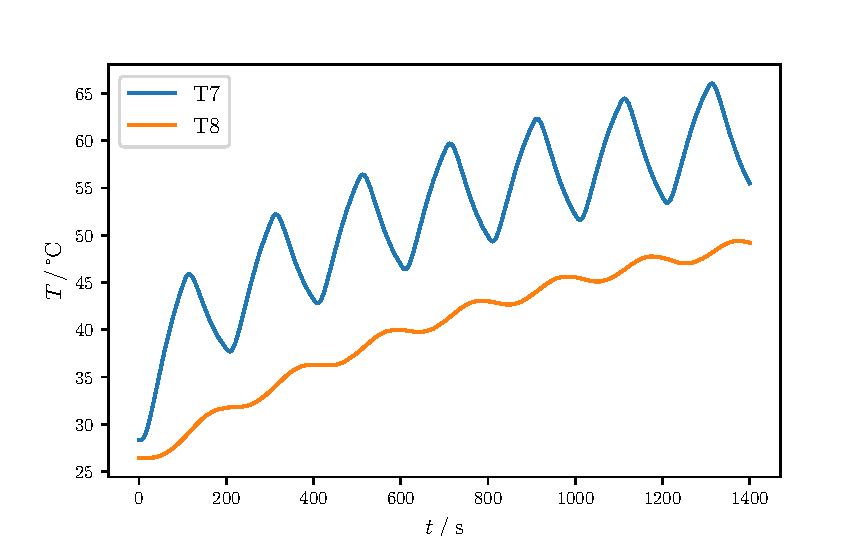
\includegraphics{plot5.pdf}
  \caption{Zeitlicher Temperaturverlauf von T7 und T8 am Edelstahlstabes bei der dynamischen Methode}
  \label{fig:g}
\end{figure}

 
  \begin{table}[H]
  \centering
    \begin{subtable}{.42\linewidth}
      \centering
        \csvreader[tabular=c c|c c|,
    head=false, 
    table head= $t\:/\:\si{\second}$ & $T_{Max}\:/\:\si{\celsius}$ & $t\:/\:\si{\second}$ & $T_{Min}\:/\si{\celsius}$\\\midrule,
    late after line= \\]
    {content/Data/Tab5.csv}{1=\eins, 2=\zwei, 3=\drei, 4=\vier}{$\num{\eins}$ & $\num{\zwei}$ & $\num{\drei}$ & $\num{\vier}$}
            \caption{Extrema bei T7}

    \end{subtable}
    \begin{subtable}{.42\linewidth}
      \centering
        \csvreader[tabular=|c c|c c,
    head=false, 
    table head= $t\:/\:\si{\second}$ & $T_{Max}\:/\:\si{\celsius}$ & $t\:/\:\si{\second}$ & $T_{Min}\:/\si{\celsius}$\\\midrule,
    late after line= \\]
    {content/Data/Tab6.csv}{1=\eins, 2=\zwei, 3=\drei, 4=\vier}{$\num{\eins}$ & $\num{\zwei}$ & $\num{\drei}$ & $\num{\vier}$}
           \caption{Extrema bei T8}

    \end{subtable} 
        \caption{Extrema der Temperaturen beim Edelstahlstab bei der dynamischen Methode}
    \label{tab:d}
\end{table}


\noindent Die Amplituden ergeben sich durch Gleichung \ref{eq:a} zu den Werten in Tabelle \ref{tab:cc}.
 
 
 \begin{table}[H]
  \centering
    \begin{subtable}{.42\linewidth}
      \centering
        \csvreader[tabular=c c,
    head=false, 
    table head= Amplitude & $T_{Max}\:/\:\si{\celsius}$\\\midrule,
    late after line= \\]
    {content/Data/Tab3_1.csv}{1=\eins, 2=\zwei}{$\num{\eins}$ & $\num{\zwei}$}
            \caption{Amplituden von T7}

    \end{subtable}
    \begin{subtable}{.42\linewidth}
      \centering
        \csvreader[tabular=c c,
    head=false, 
    table head= Amplitude & $T_{Max}\:/\:\si{\celsius}$ \\\midrule,
    late after line= \\]
    {content/Data/Tab3_2.csv}{1=\eins, 2=\zwei}{$\num{\eins}$ & $\num{\zwei}$}
           \caption{Amplituden von T8}

    \end{subtable} 
        \caption{Amplituden der Temperatur des Edelstahlstabes}
    \label{tab:cc}
\end{table}

\noindent Diese lassen sich nun mit \ref{eq:b} und \ref{eq:c} als 

\begin{equation*}
  A_{fern}=(1,01 \pm 0,08)\,\si{\celsius} 
\end{equation*}
\noindent und
\begin{equation*}
  A_{nah}=(6,02 \pm 0,09)\,\si{\celsius} 
\end{equation*}
\noindent schreiben. Die einzelnen $\delta t$ werden in Tabelle \ref{tab:ccc} aufgeführt.


\begin{table}[H]
      \centering
        \csvreader[tabular=c c,
    head=false, 
    table head= Phasendifferenz & $t\:/\:\si{\second}$\\\midrule,
    late after line= \\]
    {content/Data/Tab3_3.csv}{1=\eins, 2=\zwei}{$\num{\eins}$ & $\num{\zwei}$}

        \caption{Phasendifferenz der Temperaturmaxima beim Edelstahlstab}
    \label{tab:ccc}
\end{table}

\noindent Für $\Delta t$ gilt dann mit \ref{eq:b} und \ref{eq:c}

\begin{equation*}
  \Delta t=(75\pm5)\,\si{\second}
\end{equation*}

\noindent Um nun die Wärmeleitfähigkeit mit Gleichung \ref{eq:kappa} zu bestimmen wurde $\rho=7,9\,\si{\gram\per\centi\meter\tothe{3}}$ und $c=470\,\si{\joule\per\kilo\gram\per\kelvin}$ (siehe \cite{chemieTabelle} und \cite{chemieDichte}) angenommen.
Daraus ergibt sich dann insgesamt

\begin{equation*}
  \kappa=(12,5\pm1)\,\si{\watt\per\meter\per\kelvin}.
\end{equation*}

